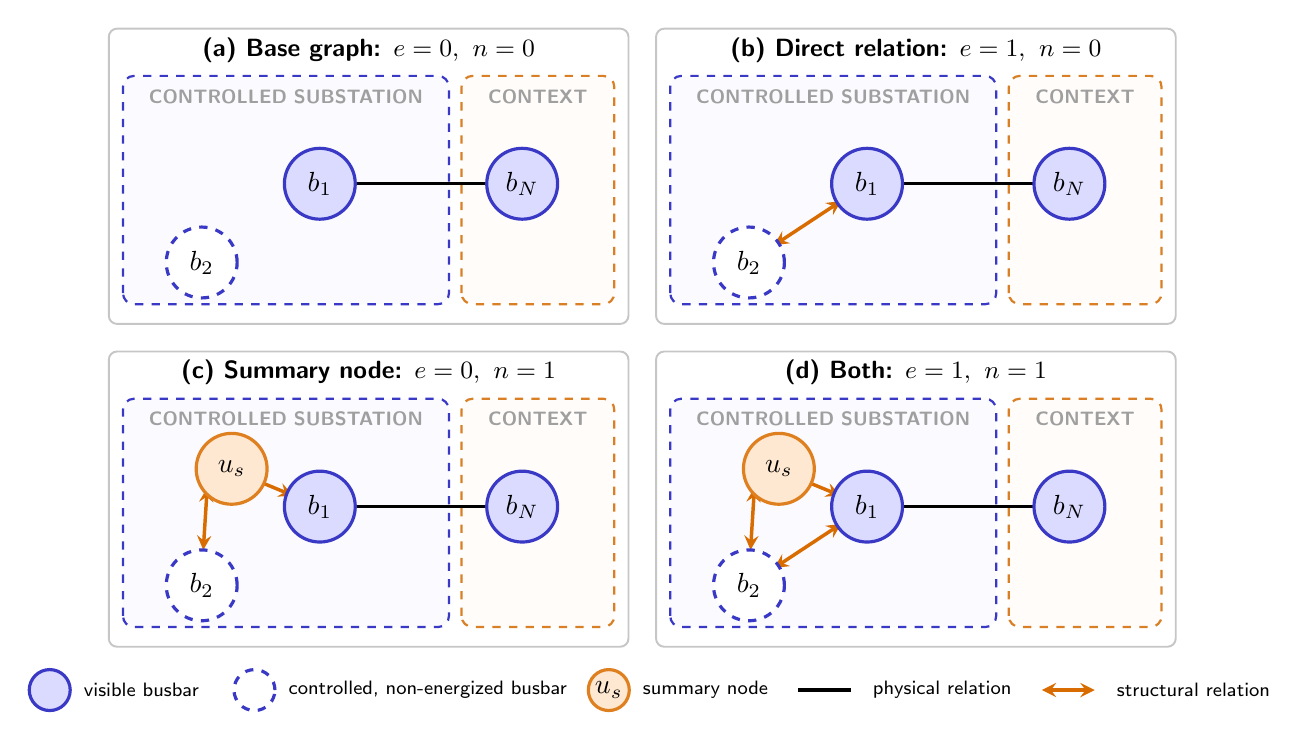
\begin{tikzpicture}[
  x=1cm,
  y=1cm,
  >=stealth,
  font=\sffamily,
  busbar/.style={
    circle,
    draw=blue!55!gray,
    fill=blue!14,
    line width=1.15pt,
    minimum size=9mm,
    inner sep=0pt
  },
  busbaroff/.style={
    circle,
    draw=blue!55!gray,
    fill=white,
    dashed,
    line width=1.15pt,
    minimum size=9mm,
    inner sep=0pt
  },
  summary/.style={
    circle,
    draw=orange!75!gray,
    fill=orange!18,
    line width=1.15pt,
    minimum size=9mm,
    inner sep=0pt
  },
  physical/.style={draw=black, line width=1.2pt},
  structural/.style={<->, draw=orange!85!black, line width=1.25pt},
  panel/.style={draw=gray!45, rounded corners=3pt, line width=0.7pt},
  controlled/.style={
    draw=blue!55!gray,
    dashed,
    rounded corners=4pt,
    fill=blue!2,
    line width=0.8pt
  },
  context/.style={
    draw=orange!70!gray,
    dashed,
    rounded corners=4pt,
    fill=orange!2,
    line width=0.8pt
  },
  zone/.style={font=\scriptsize\bfseries\sffamily, text=gray!75},
  title/.style={font=\small\bfseries\sffamily},
  legend/.style={font=\scriptsize\sffamily, align=left}
]

% A panel contains one controlled two-busbar substation and one visible
% far-end contextual busbar.  Structural augmentation is deliberately absent
% from the orange region in every case.

% ---------------------------------------------------------------------------
% (a) No augmentation
% ---------------------------------------------------------------------------
\begin{scope}[xshift=0cm,yshift=4.10cm]
  \path[panel] (0,0) rectangle (6.60,3.75);
  \node[title] at (3.30,3.48) {(a) Base graph: $e=0,\ n=0$};
  \path[controlled] (0.18,0.25) rectangle (4.32,3.15);
  \path[context] (4.48,0.25) rectangle (6.42,3.15);
  \node[zone] at (2.25,2.89) {CONTROLLED SUBSTATION};
  \node[zone] at (5.45,2.89) {CONTEXT};

  \draw[physical] (2.68,1.78) -- (5.25,1.78);
  \node[busbar] at (2.68,1.78) {$b_1$};
  \node[busbaroff] at (1.18,0.78) {$b_2$};
  \node[busbar] at (5.25,1.78) {$b_N$};
\end{scope}

% ---------------------------------------------------------------------------
% (b) Direct same-substation edge
% ---------------------------------------------------------------------------
\begin{scope}[xshift=6.95cm,yshift=4.10cm]
  \path[panel] (0,0) rectangle (6.60,3.75);
  \node[title] at (3.30,3.48) {(b) Direct relation: $e=1,\ n=0$};
  \path[controlled] (0.18,0.25) rectangle (4.32,3.15);
  \path[context] (4.48,0.25) rectangle (6.42,3.15);
  \node[zone] at (2.25,2.89) {CONTROLLED SUBSTATION};
  \node[zone] at (5.45,2.89) {CONTEXT};

  \draw[physical] (2.68,1.78) -- (5.25,1.78);
  \draw[structural] (1.50,1.00) -- (2.35,1.56);
  \node[busbar] at (2.68,1.78) {$b_1$};
  \node[busbaroff] at (1.18,0.78) {$b_2$};
  \node[busbar] at (5.25,1.78) {$b_N$};
\end{scope}

% ---------------------------------------------------------------------------
% (c) Learned substation-summary node
% ---------------------------------------------------------------------------
\begin{scope}[xshift=0cm,yshift=0cm]
  \path[panel] (0,0) rectangle (6.60,3.75);
  \node[title] at (3.30,3.48) {(c) Summary node: $e=0,\ n=1$};
  \path[controlled] (0.18,0.25) rectangle (4.32,3.15);
  \path[context] (4.48,0.25) rectangle (6.42,3.15);
  \node[zone] at (2.25,2.89) {CONTROLLED SUBSTATION};
  \node[zone] at (5.45,2.89) {CONTEXT};

  \draw[physical] (2.68,1.78) -- (5.25,1.78);
  \draw[structural] (1.54,2.25) -- (2.34,1.92);
  \draw[structural] (1.25,2.02) -- (1.20,1.23);
  \node[summary] at (1.56,2.26) {$u_s$};
  \node[busbar] at (2.68,1.78) {$b_1$};
  \node[busbaroff] at (1.18,0.78) {$b_2$};
  \node[busbar] at (5.25,1.78) {$b_N$};
\end{scope}

% ---------------------------------------------------------------------------
% (d) Both independent augmentations
% ---------------------------------------------------------------------------
\begin{scope}[xshift=6.95cm,yshift=0cm]
  \path[panel] (0,0) rectangle (6.60,3.75);
  \node[title] at (3.30,3.48) {(d) Both: $e=1,\ n=1$};
  \path[controlled] (0.18,0.25) rectangle (4.32,3.15);
  \path[context] (4.48,0.25) rectangle (6.42,3.15);
  \node[zone] at (2.25,2.89) {CONTROLLED SUBSTATION};
  \node[zone] at (5.45,2.89) {CONTEXT};

  \draw[physical] (2.68,1.78) -- (5.25,1.78);
  \draw[structural] (1.50,1.00) -- (2.35,1.56);
  \draw[structural] (1.54,2.25) -- (2.34,1.92);
  \draw[structural] (1.25,2.02) -- (1.20,1.23);
  \node[summary] at (1.56,2.26) {$u_s$};
  \node[busbar] at (2.68,1.78) {$b_1$};
  \node[busbaroff] at (1.18,0.78) {$b_2$};
  \node[busbar] at (5.25,1.78) {$b_N$};
\end{scope}

% Shared legend.
\node[busbar, minimum size=5.2mm] at (-0.75,-0.55) {};
\node[legend, anchor=west] at (-0.44,-0.55) {visible busbar};
\node[busbaroff, minimum size=5.2mm] at (1.85,-0.55) {};
\node[legend, anchor=west] at (2.16,-0.55) {controlled, non-energized busbar};
\node[summary, minimum size=5.2mm] at (6.35,-0.55) {$u_s$};
\node[legend, anchor=west] at (6.66,-0.55) {summary node};
\draw[physical] (8.75,-0.55) -- (9.42,-0.55);
\node[legend, anchor=west] at (9.58,-0.55) {physical relation};
\draw[structural] (11.85,-0.55) -- (12.52,-0.55);
\node[legend, anchor=west] at (12.68,-0.55) {structural relation};

\end{tikzpicture}
